% ==========================================
% 第二章:基于价值的强化学习
% ==========================================

\chapter{基于价值的强化学习}
\label{chap:value-based}

% ------------------------------------------
\section{引言:从价值到决策}
\label{sec:value-intro}

\subsection{核心问题}

在第一章中,我们定义了价值函数 $\Val^\policy(s)$ 和 $\Qval^\policy(s,a)$,它们衡量了给定策略 $\policy$ 下状态或状态-动作对的"好坏"。现在自然的问题是:

\begin{quote}
\textbf{如何计算价值函数?如何从价值函数导出最优策略?}
\end{quote}

这两个问题的答案构成了 Value-Based RL 的核心。本章将介绍三类方法:
\begin{enumerate}
    \item \textbf{动态规划}(Dynamic Programming):当环境模型已知时,精确求解
    \item \textbf{无模型估计}(MC 与 TD):当环境模型未知时,从采样中学习
    \item \textbf{深度 Q 网络}(DQN):处理大规模或连续状态空间
\end{enumerate}

\subsection{为什么要学习价值函数?}

一个核心观察是:\textbf{如果我们知道最优动作价值函数 $\Qval^*(s,a)$,就能直接导出最优策略}:
\begin{equation}
    \policy^*(s) = \argmax_a \Qval^*(s,a)
\end{equation}

这是 Value-Based 方法的理论基础——不直接学习策略,而是通过学习价值函数间接得到策略。

\begin{figure}[H]
    \centering
    \begin{tikzpicture}[
        box/.style={draw, rounded corners, fill=blue!10, minimum width=2.5cm, minimum height=1cm, align=center},
        arrow/.style={->, thick, >=stealth}
    ]
        % Boxes
        \node[box, fill=orange!20] (value) at (0,0) {价值函数\\$\Val^*$ 或 $\Qval^*$};
        \node[box, fill=green!20] (policy) at (5,0) {最优策略\\$\policy^*$};
        \node[box] (method) at (0,-2) {Value-Based\\方法};

        % Arrows
        \draw[arrow] (value) -- node[above] {$\argmax$} (policy);
        \draw[arrow] (method) -- (value);

        % Labels
        \node[text width=3cm, align=center, font=\footnotesize] at (-3,-2) {DP, MC, TD\\Q-Learning, DQN};
    \end{tikzpicture}
    \caption{Value-Based RL 的核心思路:学习价值函数,通过 $\argmax$ 导出策略}
    \label{fig:value-based-idea}
\end{figure}

% ------------------------------------------
\section{Bellman 方程}
\label{sec:bellman}

Bellman 方程是 RL 的核心方程,它揭示了价值函数的递推结构。理解 Bellman 方程是掌握所有 Value-Based 方法的基础。

\subsection{直觉:一步分解}

Bellman 方程的核心形式是:
\begin{equation}
    \Val^\policy(s) = \E \left[ r + \discount \Val^\policy(s') \right]
    \label{eq:bellman-intuition}
\end{equation}
用文字说:\textbf{当前状态的价值 = 即时奖励 + 折扣后的下一状态价值}。

这个递推关系使得我们可以通过迭代来计算价值函数,而不需要枚举所有可能的轨迹。

\begin{figure}[H]
    \centering
    \begin{tikzpicture}[scale=0.85]
        % Timeline
        \draw[->, thick] (0,0) -- (10,0) node[right] {时间};

        % Points
        \foreach \x/\label in {1/$t$, 4/$t+1$, 7/$t+2$} {
            \fill (\x, 0) circle (2pt);
            \node[below] at (\x, -0.2) {\label};
        }

        % Current value
        \draw[decorate, decoration={brace, amplitude=10pt, raise=5pt}] (1,0) -- (9,0)
            node[midway, above=15pt] {$\Val^\policy(s_t) = \E[G_t]$};

        % Decomposition
        \draw[decorate, decoration={brace, amplitude=8pt, raise=5pt, mirror}] (1,-0.5) -- (4,-0.5)
            node[midway, below=12pt] {$r_t$};
        \draw[decorate, decoration={brace, amplitude=8pt, raise=5pt, mirror}] (4,-0.5) -- (9,-0.5)
            node[midway, below=12pt] {$\discount \Val^\policy(s_{t+1})$};
    \end{tikzpicture}
    \caption{Bellman 方程的直觉:将无限长的回报分解为"一步奖励 + 剩余价值"}
    \label{fig:bellman-intuition}
\end{figure}

\subsection{Bellman Expectation Equation 的详细推导}

我们首先推导策略 $\policy$ 下的 Bellman Expectation Equation。

\begin{theorem}[Bellman Expectation Equation for $\Val^\policy$]
\label{thm:bellman-expectation-v}
对于任意策略 $\policy$,状态价值函数满足:
\begin{equation}
    \Val^\policy(s) = \sum_{a \in \actionspace} \policy(a|s) \left[ R(s,a) + \discount \sum_{s' \in \statespace} P(s'|s,a) \Val^\policy(s') \right]
    \label{eq:bellman-expectation-v}
\end{equation}
或写成紧凑的期望形式:
\begin{equation}
    \Val^\policy(s) = \E_{a \sim \policy, s' \sim P} \left[ R(s,a) + \discount \Val^\policy(s') \mid S_t = s \right]
\end{equation}
\end{theorem}

\begin{proof}
从状态价值函数的定义出发(回顾第一章 \eqref{eq:state-value}):
\begin{align}
    \Val^\policy(s) &= \E_\policy \left[ G_t \mid S_t = s \right] \\
    &= \E_\policy \left[ r_t + \discount G_{t+1} \mid S_t = s \right] \quad \text{(回报的递推关系 \eqref{eq:return-recursive})}
\end{align}

关键步骤:由于 $G_{t+1}$ 只依赖于 $S_{t+1}$ 之后的轨迹,我们可以条件分解:
\begin{align}
    \Val^\policy(s) &= \E_\policy \left[ r_t + \discount \E_\policy[G_{t+1} | S_{t+1}] \mid S_t = s \right] \\
    &= \E_\policy \left[ r_t + \discount \Val^\policy(S_{t+1}) \mid S_t = s \right]
\end{align}

其中最后一步使用了 $\Val^\policy(s') = \E_\policy[G_{t+1}|S_{t+1}=s']$ 的定义。

现在展开期望。由于给定 $S_t = s$:
\begin{itemize}
    \item 动作 $A_t = a$ 的概率为 $\policy(a|s)$
    \item 给定 $(s, a)$,下一状态 $S_{t+1} = s'$ 的概率为 $P(s'|s,a)$
    \item 即时奖励 $r_t = R(s,a)$(假设确定性奖励,随机情况类似)
\end{itemize}

因此:
\begin{align}
    \Val^\policy(s) &= \sum_{a \in \actionspace} \policy(a|s) \sum_{s' \in \statespace} P(s'|s,a) \left[ R(s,a) + \discount \Val^\policy(s') \right] \\
    &= \sum_{a \in \actionspace} \policy(a|s) \left[ R(s,a) + \discount \sum_{s' \in \statespace} P(s'|s,a) \Val^\policy(s') \right]
\end{align}
\end{proof}

\begin{figure}[H]
    \centering
    \begin{tikzpicture}[scale=0.9, every node/.style={scale=0.9}]
        % State s (root)
        \node[circle, draw, fill=blue!25, minimum size=1.4cm, font=\bfseries] (s) at (0,0) {$s$};
        \node[above=0.4cm of s, font=\small] {$\Val^\policy(s)$};

        % Actions (level 1)
        \node[rectangle, draw, fill=orange!25, minimum size=0.8cm] (a1) at (-3,-2) {$a_1$};
        \node[rectangle, draw, fill=orange!25, minimum size=0.8cm] (a2) at (0,-2) {$a_2$};
        \node[rectangle, draw, fill=orange!25, minimum size=0.8cm] (a3) at (3,-2) {$a_3$};

        % Policy probabilities
        \draw[->, thick, blue!70] (s) -- node[left, pos=0.6, font=\scriptsize] {$\policy(a_1|s)$} (a1);
        \draw[->, thick, blue!70] (s) -- node[right, pos=0.4, font=\scriptsize] {$\policy(a_2|s)$} (a2);
        \draw[->, thick, blue!70] (s) -- node[right, pos=0.6, font=\scriptsize] {$\policy(a_3|s)$} (a3);

        % Next states (level 2)
        \node[circle, draw, fill=blue!15, minimum size=1cm] (s11) at (-4,-4.5) {$s'_1$};
        \node[circle, draw, fill=blue!15, minimum size=1cm] (s12) at (-2,-4.5) {$s'_2$};
        \node[circle, draw, fill=blue!15, minimum size=1cm] (s21) at (-0.5,-4.5) {$s'_1$};
        \node[circle, draw, fill=blue!15, minimum size=1cm] (s22) at (1.5,-4.5) {$s'_3$};
        \node[circle, draw, fill=blue!15, minimum size=1cm] (s31) at (3,-4.5) {$s'_2$};

        % Transition probabilities and rewards
        \draw[->, dashed, gray] (a1) -- node[left, font=\tiny] {$P, R$} (s11);
        \draw[->, dashed, gray] (a1) -- node[right, font=\tiny] {$P, R$} (s12);
        \draw[->, dashed, gray] (a2) -- node[left, font=\tiny] {$P, R$} (s21);
        \draw[->, dashed, gray] (a2) -- node[right, font=\tiny] {$P, R$} (s22);
        \draw[->, dashed, gray] (a3) -- node[right, font=\tiny] {$P, R$} (s31);

        % Value labels
        \node[below=0.2cm of s11, font=\tiny] {$\discount\Val^\policy(s'_1)$};
        \node[below=0.2cm of s12, font=\tiny] {$\discount\Val^\policy(s'_2)$};

        % Legend
        \node[draw, rounded corners, fill=gray!10, font=\scriptsize, text width=4cm] at (6, -2) {
            \textbf{Backup 图说明}\\
            $\circ$ = 状态节点\\
            $\square$ = 动作节点\\
            蓝色箭头 = 策略 $\policy(a|s)$\\
            灰色虚线 = 环境转移 $P(s'|s,a)$
        };
    \end{tikzpicture}
    \caption{Bellman Expectation Equation 的 Backup 图。从状态 $s$ 出发,先按策略 $\policy(a|s)$ 选择动作,再按环境转移概率 $P(s'|s,a)$ 到达下一状态。价值"回溯"地从叶子节点传播到根节点。}
    \label{fig:bellman-backup}
\end{figure}

类似地,我们可以推导 $\Qval^\policy$ 的 Bellman Expectation Equation:

\begin{theorem}[Bellman Expectation Equation for $\Qval^\policy$]
\label{thm:bellman-expectation-q}
对于任意策略 $\policy$,动作价值函数满足:
\begin{equation}
    \Qval^\policy(s,a) = R(s,a) + \discount \sum_{s' \in \statespace} P(s'|s,a) \sum_{a' \in \actionspace} \policy(a'|s') \Qval^\policy(s',a')
    \label{eq:bellman-expectation-q}
\end{equation}
或写成期望形式:
\begin{equation}
    \Qval^\policy(s,a) = R(s,a) + \discount \E_{s' \sim P, a' \sim \policy} \left[ \Qval^\policy(s', a') \right]
\end{equation}
\end{theorem}

\begin{proof}
从动作价值函数的定义出发:
\begin{align}
    \Qval^\policy(s,a) &= \E_\policy \left[ G_t \mid S_t = s, A_t = a \right] \\
    &= \E_\policy \left[ r_t + \discount G_{t+1} \mid S_t = s, A_t = a \right] \\
    &= R(s,a) + \discount \E_\policy \left[ G_{t+1} \mid S_t = s, A_t = a \right]
\end{align}

关键步骤:由 Markov 性质,给定 $(s,a)$ 后,$G_{t+1}$ 只通过 $S_{t+1}$ 影响。对 $S_{t+1}$ 的分布求期望:
\begin{align}
    \E_\policy \left[ G_{t+1} \mid S_t = s, A_t = a \right] &= \sum_{s'} P(s'|s,a) \E_\policy \left[ G_{t+1} \mid S_{t+1} = s' \right] \\
    &= \sum_{s'} P(s'|s,a) \Val^\policy(s')
\end{align}

利用第一章的 V-Q 关系 $\Val^\policy(s') = \sum_{a'} \policy(a'|s') \Qval^\policy(s',a')$,代入得:
\begin{equation}
    \Qval^\policy(s,a) = R(s,a) + \discount \sum_{s'} P(s'|s,a) \sum_{a'} \policy(a'|s') \Qval^\policy(s',a')
\end{equation}
\end{proof}

\begin{keypoint}
$\Val^\policy$ 与 $\Qval^\policy$ 的相互表示是推导 Bellman 方程的关键:
\begin{align}
    \Val^\policy(s) &= \sum_{a} \policy(a|s) \Qval^\policy(s,a) \label{eq:v-from-q-2} \\
    \Qval^\policy(s,a) &= R(s,a) + \discount \sum_{s'} P(s'|s,a) \Val^\policy(s') \label{eq:q-from-v}
\end{align}
将 \eqref{eq:q-from-v} 代入 \eqref{eq:v-from-q-2} 得到 $\Val^\policy$ 的 Bellman 方程;将 \eqref{eq:v-from-q-2} 代入 \eqref{eq:q-from-v} 得到 $\Qval^\policy$ 的 Bellman 方程。
\end{keypoint}

\subsection{Bellman Optimality Equation 的详细推导}

最优价值函数满足 Bellman Optimality Equation。与 Expectation 版本不同,这里对动作求\textbf{最大值}而非期望。

\begin{theorem}[Bellman Optimality Equation for $\Val^*$]
\label{thm:bellman-optimality-v}
最优状态价值函数满足:
\begin{equation}
    \Val^*(s) = \max_{a \in \actionspace} \left[ R(s,a) + \discount \sum_{s' \in \statespace} P(s'|s,a) \Val^*(s') \right]
    \label{eq:bellman-optimality-v}
\end{equation}
\end{theorem}

\begin{proof}
最优价值函数的定义是所有策略中最大的价值:
\begin{equation}
    \Val^*(s) = \max_\policy \Val^\policy(s)
\end{equation}

最优策略 $\policy^*$ 是确定性的,在每个状态选择使 $\Qval^*(s,a)$ 最大的动作。因此:
\begin{align}
    \Val^*(s) &= \Val^{\policy^*}(s) \\
    &= \max_a \Qval^*(s,a) \quad \text{(最优策略选择最大 Q 值的动作)}
\end{align}

由 \eqref{eq:q-from-v} 对最优策略成立:
\begin{equation}
    \Qval^*(s,a) = R(s,a) + \discount \sum_{s'} P(s'|s,a) \Val^*(s')
\end{equation}

代入得:
\begin{equation}
    \Val^*(s) = \max_a \left[ R(s,a) + \discount \sum_{s'} P(s'|s,a) \Val^*(s') \right]
\end{equation}
\end{proof}

\begin{theorem}[Bellman Optimality Equation for $\Qval^*$]
\label{thm:bellman-optimality-q}
最优动作价值函数满足:
\begin{equation}
    \Qval^*(s,a) = R(s,a) + \discount \sum_{s' \in \statespace} P(s'|s,a) \max_{a' \in \actionspace} \Qval^*(s',a')
    \label{eq:bellman-optimality-q}
\end{equation}
\end{theorem}

\begin{proof}
\begin{align}
    \Qval^*(s,a) &= R(s,a) + \discount \sum_{s'} P(s'|s,a) \Val^*(s') \\
    &= R(s,a) + \discount \sum_{s'} P(s'|s,a) \max_{a'} \Qval^*(s',a')
\end{align}
其中最后一步使用了 $\Val^*(s') = \max_{a'} \Qval^*(s',a')$。
\end{proof}

\begin{figure}[H]
    \centering
    \begin{tikzpicture}[scale=0.85]
        % Bellman Expectation
        \begin{scope}[shift={(-4,0)}]
            \node[circle, draw, fill=blue!20, minimum size=1cm] (s1) at (0,0) {$s$};
            \node[rectangle, draw, fill=orange!20, minimum size=0.6cm] (a11) at (-1,-1.5) {$a_1$};
            \node[rectangle, draw, fill=orange!20, minimum size=0.6cm] (a12) at (1,-1.5) {$a_2$};
            \draw[->, thick] (s1) -- node[left, font=\tiny] {$\policy$} (a11);
            \draw[->, thick] (s1) -- node[right, font=\tiny] {$\policy$} (a12);
            \node[circle, draw, fill=blue!10, minimum size=0.7cm] (s11) at (-1,-3) {$s'$};
            \node[circle, draw, fill=blue!10, minimum size=0.7cm] (s12) at (1,-3) {$s'$};
            \draw[->, dashed] (a11) -- (s11);
            \draw[->, dashed] (a12) -- (s12);
            \node[below=0.3cm of s1, yshift=-3.8cm, font=\small] {Bellman Expectation};
            \node[below=0.3cm of s1, yshift=-4.5cm, font=\scriptsize] {$\sum_a \policy(a|s) [\cdots]$};
        \end{scope}

        % Bellman Optimality
        \begin{scope}[shift={(4,0)}]
            \node[circle, draw, fill=blue!20, minimum size=1cm] (s2) at (0,0) {$s$};
            \node[rectangle, draw, fill=green!30, minimum size=0.6cm] (a21) at (-1,-1.5) {$a_1$};
            \node[rectangle, draw, fill=orange!20, minimum size=0.6cm] (a22) at (1,-1.5) {$a_2$};
            \draw[->, thick, green!60!black] (s2) -- node[left, font=\tiny] {$\max$} (a21);
            \draw[->, thick, gray] (s2) -- (a22);
            \node[circle, draw, fill=blue!10, minimum size=0.7cm] (s21) at (-1,-3) {$s'$};
            \node[circle, draw, fill=blue!10, minimum size=0.7cm] (s22) at (1,-3) {$s'$};
            \draw[->, dashed] (a21) -- (s21);
            \draw[->, dashed] (a22) -- (s22);
            \node[below=0.3cm of s2, yshift=-3.8cm, font=\small] {Bellman Optimality};
            \node[below=0.3cm of s2, yshift=-4.5cm, font=\scriptsize] {$\max_a [\cdots]$};
        \end{scope}

        % VS
        \node[font=\Large] at (0, -1.5) {vs};
    \end{tikzpicture}
    \caption{Bellman Expectation vs. Bellman Optimality。左图对动作求加权平均(按 $\policy$),右图对动作求最大值。}
    \label{fig:bellman-comparison}
\end{figure}

\begin{important}
Bellman Expectation vs. Bellman Optimality 的关键区别:
\begin{itemize}
    \item \textbf{Bellman Expectation}:对动作求加权平均(按 $\policy(a|s)$),描述\textbf{给定策略}的价值
    \item \textbf{Bellman Optimality}:对动作求最大值($\max_a$),描述\textbf{最优策略}的价值
\end{itemize}
\textbf{Q-Learning 直接逼近 $\Qval^*$,因此使用 Bellman Optimality Equation 作为更新目标}。
\end{important}

\subsection{$\Val^*$ 与 $\Qval^*$ 的关系}

最优价值函数之间的关系:
\begin{align}
    \Val^*(s) &= \max_a \Qval^*(s,a) \\
    \Qval^*(s,a) &= R(s,a) + \discount \sum_{s'} P(s'|s,a) \Val^*(s')
\end{align}

由 $\Qval^*$ 可以直接导出最优策略:
\begin{equation}
    \policy^*(s) = \argmax_a \Qval^*(s,a)
\end{equation}

这是 Q-Learning 系列方法的理论基础:\textbf{只要学到 $\Qval^*$,就能得到最优策略}。

\subsection{Bellman 算子与收缩性质}

为了理解为什么基于 Bellman 方程的迭代方法能够收敛,我们引入 Bellman 算子的概念。

\begin{definition}[Bellman 算子]
定义 Bellman Expectation 算子 $\mathcal{T}^\policy$ 和 Bellman Optimality 算子 $\mathcal{T}^*$:
\begin{align}
    (\mathcal{T}^\policy \Val)(s) &= \sum_a \policy(a|s) \left[ R(s,a) + \discount \sum_{s'} P(s'|s,a) \Val(s') \right] \\
    (\mathcal{T}^* \Val)(s) &= \max_a \left[ R(s,a) + \discount \sum_{s'} P(s'|s,a) \Val(s') \right]
\end{align}
\end{definition}

\begin{theorem}[Bellman 算子的收缩性]
\label{thm:bellman-contraction}
Bellman 算子是 $\gamma$-收缩映射。即对于任意两个价值函数 $\Val_1, \Val_2$:
\begin{equation}
    \| \mathcal{T}^\policy \Val_1 - \mathcal{T}^\policy \Val_2 \|_\infty \leq \discount \| \Val_1 - \Val_2 \|_\infty
\end{equation}
$\mathcal{T}^*$ 同样满足此性质。
\end{theorem}

\begin{proof}
对于任意状态 $s$:
\begin{align}
    |(\mathcal{T}^\policy \Val_1)(s) - (\mathcal{T}^\policy \Val_2)(s)| &= \left| \discount \sum_a \policy(a|s) \sum_{s'} P(s'|s,a) [\Val_1(s') - \Val_2(s')] \right| \\
    &\leq \discount \sum_a \policy(a|s) \sum_{s'} P(s'|s,a) |\Val_1(s') - \Val_2(s')| \\
    &\leq \discount \| \Val_1 - \Val_2 \|_\infty \underbrace{\sum_a \policy(a|s) \sum_{s'} P(s'|s,a)}_{=1} \\
    &= \discount \| \Val_1 - \Val_2 \|_\infty
\end{align}
对所有 $s$ 取最大,得到结论。
\end{proof}

\begin{keypoint}
收缩性质的重要推论:
\begin{enumerate}
    \item \textbf{唯一不动点}:Bellman 算子有唯一的不动点 $\Val^\policy$(或 $\Val^*$)
    \item \textbf{迭代收敛}:从任意初始 $\Val_0$ 出发,$\Val_{k+1} = \mathcal{T}\Val_k$ 收敛到不动点
    \item \textbf{收敛速度}:误差以 $\discount^k$ 的速度指数衰减
\end{enumerate}
\end{keypoint}

% ------------------------------------------
\section{动态规划方法}
\label{sec:dp}

当环境模型 $P(s'|s,a)$ 和 $R(s,a)$ 完全已知时,可以使用动态规划(Dynamic Programming, DP)方法精确求解最优策略。

\subsection{Policy Evaluation(策略评估)}

给定策略 $\policy$,如何计算其价值函数 $\Val^\policy$?

\begin{definition}[Policy Evaluation]
Policy Evaluation 是通过迭代 Bellman Expectation 方程来计算 $\Val^\policy$ 的过程:
\begin{equation}
    \Val_{k+1}(s) = \sum_a \policy(a|s) \left[ R(s,a) + \discount \sum_{s'} P(s'|s,a) \Val_k(s') \right]
    \label{eq:policy-eval-update}
\end{equation}
从任意初始 $\Val_0$ 开始,迭代直到收敛 $\Val_k \to \Val^\policy$。
\end{definition}

\begin{theorem}[Policy Evaluation 的收敛性]
\label{thm:policy-eval-convergence}
对于任意初始 $\Val_0$ 和 $\discount < 1$,Policy Evaluation 迭代收敛到唯一的 $\Val^\policy$。收敛速度为 $O(\discount^k)$。
\end{theorem}

\begin{proof}
由定理 \ref{thm:bellman-contraction},Bellman 算子 $\mathcal{T}^\policy$ 是 $\gamma$-收缩映射。由 Banach 不动点定理:
\begin{enumerate}
    \item 存在唯一不动点 $\Val^\policy$ 使得 $\mathcal{T}^\policy \Val^\policy = \Val^\policy$
    \item 对任意 $\Val_0$,序列 $\Val_{k+1} = \mathcal{T}^\policy \Val_k$ 收敛到 $\Val^\policy$
\end{enumerate}

误差界:$\|\Val_k - \Val^\policy\|_\infty \leq \discount^k \|\Val_0 - \Val^\policy\|_\infty$
\end{proof}

\begin{algorithm}[H]
\caption{Policy Evaluation}
\label{alg:policy-evaluation}
\KwInput{策略 $\policy$,MDP $(\statespace, \actionspace, P, R, \discount)$,收敛阈值 $\theta$}
\KwOutput{价值函数 $\Val^\policy$}
初始化 $\Val(s) = 0$ 对于所有 $s \in \statespace$\;
\Repeat{$\Delta < \theta$}{
    $\Delta \leftarrow 0$\;
    \ForEach{$s \in \statespace$}{
        $v \leftarrow \Val(s)$\;
        $\Val(s) \leftarrow \sum_a \policy(a|s) \left[ R(s,a) + \discount \sum_{s'} P(s'|s,a) \Val(s') \right]$\;
        $\Delta \leftarrow \max(\Delta, |v - \Val(s)|)$\;
    }
}
\Return{$\Val$}
\end{algorithm}

\subsection{Policy Improvement(策略改进)}

给定 $\Val^\policy$,如何构造一个更好的策略?

\begin{theorem}[Policy Improvement Theorem]
\label{thm:policy-improvement}
设 $\policy$ 和 $\policy'$ 是两个策略。如果对于所有 $s \in \statespace$:
\begin{equation}
    \Qval^\policy(s, \policy'(s)) \geq \Val^\policy(s)
    \label{eq:policy-improvement-condition}
\end{equation}
则 $\policy'$ 至少与 $\policy$ 一样好:对于所有 $s$,$\Val^{\policy'}(s) \geq \Val^\policy(s)$。
\end{theorem}

\begin{proof}
从条件 \eqref{eq:policy-improvement-condition} 出发,利用 $\Qval^\policy$ 的定义展开:
\begin{align}
    \Val^\policy(s) &\leq \Qval^\policy(s, \policy'(s)) \\
    &= R(s, \policy'(s)) + \discount \sum_{s'} P(s'|s, \policy'(s)) \Val^\policy(s') \\
    &\leq R(s, \policy'(s)) + \discount \sum_{s'} P(s'|s, \policy'(s)) \Qval^\policy(s', \policy'(s')) \quad \text{(再用条件)}\\
    &= R(s, \policy'(s)) + \discount \sum_{s'} P(s'|s, \policy'(s)) \left[ R(s', \policy'(s')) + \discount \sum_{s''} P(s''|s', \policy'(s')) \Val^\policy(s'') \right]
\end{align}

继续展开,直到 episode 结束(或利用折扣因子使尾部趋近于零):
\begin{align}
    \Val^\policy(s) &\leq \E_{\policy'} \left[ r_0 + \discount r_1 + \discount^2 r_2 + \cdots \mid S_0 = s \right] \\
    &= \Val^{\policy'}(s)
\end{align}
\end{proof}

\begin{note}
Policy Improvement Theorem 的直觉:如果在每个状态,按 $\policy'$ 选择动作比按 $\policy$ 选择更好(体现在 Q 值上),那么整体策略 $\policy'$ 也更好。
\end{note}

贪心策略改进保证了条件 \eqref{eq:policy-improvement-condition} 以等号或严格大于成立:

\begin{definition}[贪心策略改进]
给定 $\Val^\policy$,定义贪心改进策略:
\begin{equation}
    \policy'(s) = \argmax_a \Qval^\policy(s,a) = \argmax_a \left[ R(s,a) + \discount \sum_{s'} P(s'|s,a) \Val^\policy(s') \right]
    \label{eq:greedy-improvement}
\end{equation}
\end{definition}

对于贪心改进:
\begin{equation}
    \Qval^\policy(s, \policy'(s)) = \max_a \Qval^\policy(s, a) \geq \Qval^\policy(s, \policy(s)) = \Val^\policy(s)
\end{equation}
因此满足 Policy Improvement Theorem 的条件。

\subsection{Policy Iteration}

交替进行 Policy Evaluation 和 Policy Improvement:

\begin{figure}[H]
    \centering
    \begin{tikzpicture}[
        box/.style={draw, rounded corners, fill=blue!15, minimum width=2cm, minimum height=0.8cm, align=center},
        arrow/.style={->, thick, >=stealth}
    ]
        % Boxes
        \node[box] (pi1) at (0,0) {$\policy_0$};
        \node[box, fill=green!15] (v1) at (2.5,0) {$\Val^{\policy_0}$};
        \node[box] (pi2) at (5,0) {$\policy_1$};
        \node[box, fill=green!15] (v2) at (7.5,0) {$\Val^{\policy_1}$};
        \node[box] (pi3) at (10,0) {$\policy_2$};
        \node at (11.5, 0) {$\cdots$};

        % Arrows - 使用 yshift 上移标签避免被节点遮挡
        \draw[arrow] (pi1) -- node[above, font=\scriptsize, yshift=6pt] {Eval} (v1);
        \draw[arrow] (v1) -- node[above, font=\scriptsize, yshift=6pt] {Improve} (pi2);
        \draw[arrow] (pi2) -- node[above, font=\scriptsize, yshift=6pt] {Eval} (v2);
        \draw[arrow] (v2) -- node[above, font=\scriptsize, yshift=6pt] {Improve} (pi3);

        % Labels
        \node[below=0.5cm of v1, font=\small, text=gray] {完整求解};
        \node[below=0.5cm of pi2, font=\small, text=gray] {贪心};
    \end{tikzpicture}
    \caption{Policy Iteration 的流程:评估 $\to$ 改进 $\to$ 评估 $\to$ 改进 $\to$ $\cdots$}
    \label{fig:policy-iteration}
\end{figure}

\begin{algorithm}[H]
\caption{Policy Iteration}
\label{alg:policy-iteration}
\KwInput{MDP $(\statespace, \actionspace, P, R, \discount)$}
\KwOutput{最优策略 $\policy^*$ 和最优价值 $\Val^*$}
初始化 $\policy$ 为任意策略\;
\Repeat{$\policy$ 不再改变(policy-stable = true)}{
    \textbf{Policy Evaluation}: 计算 $\Val^\policy$(使用算法 \ref{alg:policy-evaluation})\;
    policy-stable $\leftarrow$ true\;
    \ForEach{$s \in \statespace$}{
        old-action $\leftarrow \policy(s)$\;
        $\policy(s) \leftarrow \argmax_a \left[ R(s,a) + \discount \sum_{s'} P(s'|s,a) \Val^\policy(s') \right]$\;
        \If{old-action $\neq \policy(s)$}{
            policy-stable $\leftarrow$ false\;
        }
    }
}
\Return{$\policy, \Val^\policy$}
\end{algorithm}

\begin{theorem}[Policy Iteration 的有限步收敛]
对于有限 MDP,Policy Iteration 在有限步内收敛到最优策略 $\policy^*$。
\end{theorem}

\begin{proof}
\begin{enumerate}
    \item 由 Policy Improvement Theorem,每次迭代 $\Val^{\policy_{k+1}}(s) \geq \Val^{\policy_k}(s)$ 对所有 $s$ 成立
    \item 有限 MDP 只有有限多个确定性策略($|\actionspace|^{|\statespace|}$ 个)
    \item 价值函数严格单调递增(除非已是最优),因此不会循环
    \item 结合上述,必在有限步内收敛
\end{enumerate}
\end{proof}

\subsection{Value Iteration}

Value Iteration 将 Policy Evaluation 和 Policy Improvement 合并为一步,直接迭代 Bellman Optimality 方程:

\begin{algorithm}[H]
\caption{Value Iteration}
\label{alg:value-iteration}
\KwInput{MDP $(\statespace, \actionspace, P, R, \discount)$, 收敛阈值 $\theta$}
\KwOutput{最优价值 $\Val^*$ 和最优策略 $\policy^*$}
初始化 $\Val(s) = 0$ 对于所有 $s$\;
\Repeat{$\Delta < \theta$}{
    $\Delta \leftarrow 0$\;
    \ForEach{$s \in \statespace$}{
        $v \leftarrow \Val(s)$\;
        $\Val(s) \leftarrow \max_a \left[ R(s,a) + \discount \sum_{s'} P(s'|s,a) \Val(s') \right]$\;
        $\Delta \leftarrow \max(\Delta, |v - \Val(s)|)$\;
    }
}
$\policy^*(s) \leftarrow \argmax_a \left[ R(s,a) + \discount \sum_{s'} P(s'|s,a) \Val(s') \right]$ 对于所有 $s$\;
\Return{$\Val, \policy^*$}
\end{algorithm}

\begin{keypoint}
Value Iteration vs. Policy Iteration 的对比:

\begin{table}[H]
    \centering
    \begin{tabular}{@{}lcc@{}}
        \toprule
        & \textbf{Policy Iteration} & \textbf{Value Iteration} \\
        \midrule
        Policy Evaluation & 完整求解 $\Val^\policy$ & 仅一步 Bellman 更新 \\
        理论依据 & Bellman Expectation & Bellman Optimality \\
        每轮复杂度 & 高(需多次内循环) & 低(单次遍历) \\
        收敛轮数 & 少 & 多 \\
        总体效率 & 较低 & 通常更高 \\
        \bottomrule
    \end{tabular}
\end{table}

实践中,Value Iteration 通常更高效,因为不需要在每轮完整求解 $\Val^\policy$。
\end{keypoint}

\subsection{DP 方法的局限性}

动态规划虽然能精确求解,但有明显局限:
\begin{enumerate}
    \item \textbf{需要完整模型}:必须知道 $P(s'|s,a)$ 和 $R(s,a)$
    \item \textbf{状态空间遍历}:每轮需要遍历所有状态,复杂度 $O(|\statespace|^2 |\actionspace|)$
    \item \textbf{无法处理连续空间}:表格方法无法直接应用
\end{enumerate}

这些局限促使了无模型方法(MC、TD)和函数逼近方法(DQN)的发展。

% ------------------------------------------
\section{无模型方法:Monte Carlo vs Temporal Difference}
\label{sec:mc-td}

当环境模型未知时,需要通过与环境交互的样本来估计价值函数。两种主要方法是 Monte Carlo (MC) 和 Temporal Difference (TD)。

\subsection{核心问题}

\begin{quote}
\textbf{只有采样数据,没有环境模型 $P$ 和 $R$,如何估计 $\Val^\policy(s)$?}
\end{quote}

回顾价值函数的定义:
\begin{equation}
    \Val^\policy(s) = \E_\policy[G_t | S_t = s]
\end{equation}

这是一个期望,可以用样本均值来估计。

\subsection{Monte Carlo 估计}

MC 方法的核心思想:\textbf{用实际轨迹的回报 $G_t$ 来估计期望}。

\begin{definition}[Monte Carlo 更新]
对于在轨迹中访问过的状态 $S_t$:
\begin{equation}
    \Val(S_t) \leftarrow \Val(S_t) + \alpha \left( G_t - \Val(S_t) \right)
    \label{eq:mc-update}
\end{equation}
其中 $G_t = \sum_{k=0}^{T-t-1} \discount^k r_{t+k}$ 是从 $t$ 时刻开始到 episode 结束的实际回报,$\alpha$ 是学习率。
\end{definition}

\begin{note}
MC 更新可以理解为增量式均值估计。如果 $\alpha = 1/N(s)$($N(s)$ 是状态 $s$ 的访问次数),则 $\Val(s)$ 正好是历史回报的均值。
\end{note}

MC 方法的特点:
\begin{itemize}
    \item \textbf{必须等到 episode 结束}才能计算 $G_t$,仅适用于 episodic 任务
    \item \textbf{无偏估计}:$\E[G_t | S_t = s] = \Val^\policy(s)$,不依赖任何估计值
    \item \textbf{高方差}:$G_t$ 累积了整条轨迹的随机性(动作选择、状态转移、奖励)
    \item \textbf{不使用 Bootstrap}:目标完全来自真实采样
\end{itemize}

\subsection{Temporal Difference 估计}

TD 方法的核心思想:\textbf{用"一步奖励 + 下一状态的估计价值"来代替完整回报}。

\begin{definition}[TD(0) 更新]
对于每一步转移 $(S_t, A_t, R_t, S_{t+1})$:
\begin{equation}
    \Val(S_t) \leftarrow \Val(S_t) + \alpha \left( \underbrace{r_t + \discount \Val(S_{t+1})}_{\text{TD target}} - \Val(S_t) \right)
    \label{eq:td-update}
\end{equation}
其中 TD 误差定义为:
\begin{equation}
    \delta_t = r_t + \discount \Val(S_{t+1}) - \Val(S_t)
    \label{eq:td-error}
\end{equation}
\end{definition}

TD 方法的特点:
\begin{itemize}
    \item \textbf{每步都可更新},适用于 continuing 任务和在线学习
    \item \textbf{有偏估计}:使用了 $\Val(S_{t+1})$ 的估计值(可能不准确)
    \item \textbf{低方差}:只使用单步奖励,不累积长期随机性
    \item \textbf{使用 Bootstrap}:用当前估计 $\Val(S_{t+1})$ 来更新 $\Val(S_t)$
\end{itemize}

\begin{figure}[H]
    \centering
    \begin{tikzpicture}[scale=0.9]
        % MC
        \begin{scope}[shift={(-5,0)}]
            \node[font=\bfseries] at (0, 1.5) {Monte Carlo};
            \draw[->, thick] (0,0) -- (6,0);
            \foreach \x in {0,1,2,3,4,5} {
                \fill (\x, 0) circle (2pt);
            }
            \node[below, font=\scriptsize] at (0,0) {$S_t$};
            \node[below, font=\scriptsize] at (5,0) {$S_T$(终止)};

            \draw[decorate, decoration={brace, amplitude=5pt, raise=3pt}] (0,0) -- (5,0)
                node[midway, above=8pt, font=\scriptsize] {$G_t = r_t + \gamma r_{t+1} + \cdots + \gamma^{T-t-1}r_{T-1}$};

            \node[draw, rounded corners, fill=red!20, font=\scriptsize] at (2.5, -1.2) {必须等到 episode 结束};
        \end{scope}

        % TD
        \begin{scope}[shift={(4,0)}]
            \node[font=\bfseries] at (0, 1.5) {Temporal Difference};
            \draw[->, thick] (0,0) -- (6,0);
            \foreach \x in {0,1,2,3,4,5} {
                \fill (\x, 0) circle (2pt);
            }
            \node[below, font=\scriptsize] at (0,0) {$S_t$};
            \node[below, font=\scriptsize] at (1,0) {$S_{t+1}$};

            \draw[decorate, decoration={brace, amplitude=5pt, raise=3pt}] (0,0) -- (1,0)
                node[midway, above=8pt, font=\scriptsize] {$r_t + \gamma \Val(S_{t+1})$};

            \node[draw, rounded corners, fill=green!20, font=\scriptsize] at (2.5, -1.2) {每步即可更新};
        \end{scope}
    \end{tikzpicture}
    \caption{MC 与 TD 的更新范围对比。MC 需要完整轨迹,TD 只需单步转移。}
    \label{fig:mc-td-scope}
\end{figure}

\subsection{偏差-方差权衡分析}

MC 和 TD 代表了偏差-方差权衡的两个极端。

\begin{table}[H]
    \centering
    \begin{tabular}{@{}lcc@{}}
        \toprule
        & \textbf{Monte Carlo} & \textbf{TD(0)} \\
        \midrule
        目标 & $G_t$ (真实回报) & $r_t + \discount \Val(S_{t+1})$ \\
        偏差 & 无偏 & 有偏(依赖 $\Val$ 估计) \\
        方差 & 高(累积轨迹随机性) & 低(仅单步随机性) \\
        Bootstrap & 否 & 是 \\
        适用任务 & 仅 Episodic & Episodic 和 Continuing \\
        数据效率 & 低(需完整轨迹) & 高(每步更新) \\
        \bottomrule
    \end{tabular}
    \caption{MC 与 TD 的全面对比}
    \label{tab:mc-td-comparison}
\end{table}

\begin{keypoint}
为什么 TD 方差更小?

MC 目标 $G_t = r_t + \discount r_{t+1} + \discount^2 r_{t+2} + \cdots$ 包含了从 $t$ 到终止的所有奖励。每个 $r_k$ 都是随机变量(取决于策略选择和环境转移),方差叠加:
\begin{equation}
    \text{Var}(G_t) = \sum_{k=0}^{T-t-1} \discount^{2k} \text{Var}(r_{t+k}) + \text{协方差项}
\end{equation}

TD 目标 $r_t + \discount \Val(S_{t+1})$ 只有 $r_t$ 和 $S_{t+1}$ 是随机的。虽然 $\Val(S_{t+1})$ 可能不准确(有偏),但它是一个相对平滑的函数估计,不会累积随机性。
\end{keypoint}

\begin{figure}[H]
    \centering
    \begin{tikzpicture}
        \begin{axis}[
            width=10cm, height=6cm,
            xlabel={偏差},
            ylabel={方差},
            xmin=-0.5, xmax=3.5,
            ymin=-0.5, ymax=3.2,
            axis lines=middle,
            xtick=\empty, ytick=\empty,
            clip=false
        ]
        % Points with adjusted label positions - MC 右移避开 Y 轴标签
        \node[circle, fill=red!70, minimum size=8pt] (mc) at (axis cs:0.5,2.5) {};
        \node[font=\small, anchor=west] at (axis cs:0.65,2.5) {MC};

        \node[circle, fill=blue!70, minimum size=8pt] (td) at (axis cs:1.5,0.8) {};
        \node[font=\small, anchor=north] at (axis cs:1.5,0.6) {TD(0)};

        \node[circle, fill=green!70, minimum size=8pt] (nstep) at (axis cs:0.8,1.5) {};
        \node[font=\small, anchor=south west] at (axis cs:0.9,1.6) {n-step TD};

        % Arrow - 从 MC 到 TD(0)
        \draw[->, thick, dashed, gray] (axis cs:0.4,2.4) to[bend right=20] (axis cs:1.4,0.9);
        \node[font=\scriptsize, gray, anchor=west] at (axis cs:1.5, 2.2) {增加 Bootstrap};

        % MSE contours (schematic)
        \draw[gray, thin] (axis cs:0.6,1.2) ellipse [x radius=0.8, y radius=0.6];
        \node[font=\tiny, gray, anchor=west] at (axis cs:1.5, 1.2) {MSE 等高线};
        \end{axis}
    \end{tikzpicture}
    \caption{偏差-方差权衡示意图。MC 无偏但高方差,TD 有偏但低方差。n-step TD 在两者之间取得平衡。}
    \label{fig:bias-variance}
\end{figure}

\subsection{n-step TD 与 TD($\lambda$)}

n-step TD 是 MC 和 TD(0) 的中间形式,提供了在偏差-方差之间灵活权衡的方法。

\begin{definition}[n-step Return]
\begin{equation}
    G_t^{(n)} = r_t + \discount r_{t+1} + \cdots + \discount^{n-1} r_{t+n-1} + \discount^n \Val(S_{t+n})
    \label{eq:n-step-return}
\end{equation}
\end{definition}

\begin{itemize}
    \item $n=1$:$G_t^{(1)} = r_t + \discount \Val(S_{t+1})$,即 TD(0)
    \item $n=\infty$:$G_t^{(\infty)} = r_t + \discount r_{t+1} + \cdots$,即 Monte Carlo
\end{itemize}

\begin{figure}[H]
    \centering
    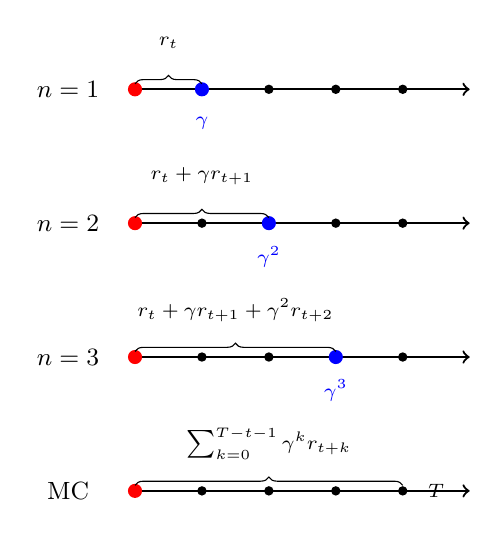
\begin{tikzpicture}[scale=0.85]
        % n=1
        \begin{scope}[shift={(0,0)}]
            \draw[->, thick] (0,0) -- (5,0);
            \foreach \x in {0,1,2,3,4} \fill (\x, 0) circle (2pt);
            \fill[red] (0,0) circle (3pt);
            \fill[blue] (1,0) circle (3pt);
            \draw[decorate, decoration={brace, amplitude=3pt, raise=2pt}] (0,0) -- (1,0);
            \node[font=\scriptsize] at (0.5, 0.7) {$r_t$};
            \node[font=\scriptsize, blue] at (1, -0.5) {$\gamma\Val$};
            \node[font=\small] at (-1, 0) {$n=1$};
        \end{scope}

        % n=2
        \begin{scope}[shift={(0,-2)}]
            \draw[->, thick] (0,0) -- (5,0);
            \foreach \x in {0,1,2,3,4} \fill (\x, 0) circle (2pt);
            \fill[red] (0,0) circle (3pt);
            \fill[blue] (2,0) circle (3pt);
            \draw[decorate, decoration={brace, amplitude=3pt, raise=2pt}] (0,0) -- (2,0);
            \node[font=\scriptsize] at (1, 0.7) {$r_t + \gamma r_{t+1}$};
            \node[font=\scriptsize, blue] at (2, -0.5) {$\gamma^2\Val$};
            \node[font=\small] at (-1, 0) {$n=2$};
        \end{scope}

        % n=3
        \begin{scope}[shift={(0,-4)}]
            \draw[->, thick] (0,0) -- (5,0);
            \foreach \x in {0,1,2,3,4} \fill (\x, 0) circle (2pt);
            \fill[red] (0,0) circle (3pt);
            \fill[blue] (3,0) circle (3pt);
            \draw[decorate, decoration={brace, amplitude=3pt, raise=2pt}] (0,0) -- (3,0);
            \node[font=\scriptsize] at (1.5, 0.7) {$r_t + \gamma r_{t+1} + \gamma^2 r_{t+2}$};
            \node[font=\scriptsize, blue] at (3, -0.5) {$\gamma^3\Val$};
            \node[font=\small] at (-1, 0) {$n=3$};
        \end{scope}

        % MC
        \begin{scope}[shift={(0,-6)}]
            \draw[->, thick] (0,0) -- (5,0);
            \foreach \x in {0,1,2,3,4} \fill (\x, 0) circle (2pt);
            \fill[red] (0,0) circle (3pt);
            \node[font=\scriptsize] at (4.5, 0) {$T$};
            \draw[decorate, decoration={brace, amplitude=3pt, raise=2pt}] (0,0) -- (4,0);
            \node[font=\scriptsize] at (2, 0.7) {$\sum_{k=0}^{T-t-1} \gamma^k r_{t+k}$};
            \node[font=\small] at (-1, 0) {MC};
        \end{scope}
    \end{tikzpicture}
    \caption{不同 $n$ 值下的 n-step return。红点为当前状态,蓝点为 Bootstrap 位置。}
    \label{fig:n-step-returns}
\end{figure}

\subsubsection{TD($\lambda$):加权平均}

TD($\lambda$) 方法将所有 n-step return 加权平均,而不是选择单一的 $n$:

\begin{definition}[$\lambda$-return]
\begin{equation}
    G_t^\lambda = (1-\lambda) \sum_{n=1}^{\infty} \lambda^{n-1} G_t^{(n)}
    \label{eq:lambda-return}
\end{equation}
其中 $\lambda \in [0,1]$ 控制权重的衰减速度。
\end{definition}

权重分布的直觉:
\begin{itemize}
    \item $G_t^{(1)}$ 的权重:$(1-\lambda)$
    \item $G_t^{(2)}$ 的权重:$(1-\lambda)\lambda$
    \item $G_t^{(n)}$ 的权重:$(1-\lambda)\lambda^{n-1}$
    \item 权重之和为 1
\end{itemize}

\begin{figure}[H]
    \centering
    \begin{tikzpicture}
        \begin{axis}[
            width=10cm, height=5cm,
            ybar,
            xlabel={$n$},
            ylabel={权重},
            symbolic x coords={1,2,3,4,5,$\cdots$,MC},
            xtick=data,
            ymin=0, ymax=0.6,
            bar width=12pt,
            nodes near coords,
            nodes near coords style={font=\tiny},
            every node near coord/.append style={yshift=3pt}
        ]
        % lambda = 0.5
        \addplot[fill=blue!60] coordinates {(1,0.5) (2,0.25) (3,0.125) (4,0.0625) (5,0.03125) ($\cdots$,0) (MC,0.03125)};
        \end{axis}
    \end{tikzpicture}
    \caption{$\lambda$-return 的权重分布($\lambda=0.5$)。短期 return 权重大,长期 return 权重指数衰减。}
    \label{fig:lambda-weights}
\end{figure}

特殊情况:
\begin{itemize}
    \item $\lambda = 0$:$G_t^\lambda = G_t^{(1)}$,等价于 TD(0)
    \item $\lambda = 1$:$G_t^\lambda = G_t^{(\infty)}$,等价于 Monte Carlo
\end{itemize}

\subsubsection{Eligibility Traces}

直接计算 $G_t^\lambda$ 需要等到 episode 结束。Eligibility Traces 提供了一种在线计算的方式。

\begin{definition}[Eligibility Trace]
为每个状态维护一个 eligibility trace $e_t(s)$:
\begin{equation}
    e_t(s) = \begin{cases}
        \gamma \lambda e_{t-1}(s) + 1 & \text{if } s = S_t \\
        \gamma \lambda e_{t-1}(s) & \text{otherwise}
    \end{cases}
\end{equation}
初始时 $e_0(s) = 0$ 对所有 $s$。
\end{definition}

TD($\lambda$) 的在线更新:
\begin{equation}
    \Val(s) \leftarrow \Val(s) + \alpha \delta_t e_t(s), \quad \forall s
\end{equation}
其中 $\delta_t = r_t + \gamma \Val(S_{t+1}) - \Val(S_t)$ 是 TD 误差。

\begin{keypoint}
Eligibility Trace 的直觉:
\begin{itemize}
    \item $e_t(s)$ 表示状态 $s$ 对当前 TD 误差的"责任"
    \item 刚访问过的状态责任大,随时间指数衰减
    \item 当 $\delta_t \neq 0$ 时,所有有责任的状态都被更新
\end{itemize}
这实现了"信用分配":奖励信号向过去的状态传播。
\end{keypoint}

% ------------------------------------------
\section{Q-Learning 与 SARSA}
\label{sec:q-learning-sarsa}

前面讨论的 MC 和 TD 方法是对 $\Val^\policy$ 的估计。为了找到最优策略,我们需要估计动作价值函数 $\Qval$,这样才能通过 $\argmax$ 导出策略。

\subsection{On-policy vs Off-policy}

\begin{definition}[On-policy 与 Off-policy]
\leavevmode
\begin{itemize}
    \item \textbf{On-policy}:评估和改进的是同一个策略
    \begin{itemize}
        \item 行为策略(收集数据)= 目标策略(被评估/改进)
        \item 例子:SARSA
    \end{itemize}
    \item \textbf{Off-policy}:用行为策略收集数据,评估/改进不同的目标策略
    \begin{itemize}
        \item 行为策略(收集数据)$\neq$ 目标策略(被评估/改进)
        \item 例子:Q-Learning
    \end{itemize}
\end{itemize}
\end{definition}

\begin{figure}[H]
    \centering
    \begin{tikzpicture}[
        box/.style={draw, rounded corners, minimum width=2cm, minimum height=1cm, align=center},
        arrow/.style={->, thick}
    ]
        % On-policy
        \begin{scope}[shift={(-4,0)}]
            \node[font=\bfseries] at (0, 2) {On-policy};
            \node[box, fill=blue!20] (behavior1) at (0, 0.5) {行为策略\\$\policy$};
            \node[box, fill=blue!20] (target1) at (0, -1.5) {目标策略\\$\policy$};
            \draw[arrow, <->] (behavior1) -- node[right, font=\scriptsize] {相同} (target1);
        \end{scope}

        % Off-policy
        \begin{scope}[shift={(4,0)}]
            \node[font=\bfseries] at (0, 2) {Off-policy};
            \node[box, fill=orange!20] (behavior2) at (-1.5, 0.5) {行为策略\\$\mu$};
            \node[box, fill=green!20] (target2) at (1.5, 0.5) {目标策略\\$\policy$};
            \node[box, fill=gray!20] (data) at (0, -1.5) {数据};
            \draw[arrow] (behavior2) -- (data);
            \draw[arrow] (data) -- (target2);
            \node[font=\scriptsize, red] at (0, 1) {不同};
        \end{scope}
    \end{tikzpicture}
    \caption{On-policy vs Off-policy。Off-policy 方法可以从任意行为策略的数据中学习目标策略。}
    \label{fig:on-off-policy}
\end{figure}

Off-policy 的优势:
\begin{itemize}
    \item 可以从历史数据(Experience Replay)中学习
    \item 可以从人类演示或其他策略的数据中学习
    \item 可以同时学习多个目标策略
\end{itemize}

\subsection{SARSA 算法}

SARSA 是一种 On-policy TD 控制方法,名字来自更新所需的五元组 $(S_t, A_t, R_t, S_{t+1}, A_{t+1})$。

\begin{definition}[SARSA 更新]
\begin{equation}
    \Qval(S_t, A_t) \leftarrow \Qval(S_t, A_t) + \alpha \left( r_t + \discount \Qval(S_{t+1}, A_{t+1}) - \Qval(S_t, A_t) \right)
    \label{eq:sarsa-update}
\end{equation}
其中 $A_{t+1}$ 是按当前策略(如 $\epsilon$-greedy)实际采样的动作。
\end{definition}

\begin{algorithm}[H]
\caption{SARSA}
\label{alg:sarsa}
\KwInput{学习率 $\alpha$,探索率 $\epsilon$,折扣因子 $\discount$}
初始化 $\Qval(s,a)$ 为任意值,$\Qval(\text{terminal}, \cdot) = 0$\;
\ForEach{episode}{
    初始化状态 $S$\;
    用 $\epsilon$-greedy 选择动作 $A$\;
    \Repeat{$S$ 是终止状态}{
        执行 $A$,观察 $R, S'$\;
        用 $\epsilon$-greedy 选择 $A'$\;
        $\Qval(S,A) \leftarrow \Qval(S,A) + \alpha \left( R + \discount \Qval(S',A') - \Qval(S,A) \right)$\;
        $S \leftarrow S'$, $A \leftarrow A'$\;
    }
}
\end{algorithm}

SARSA 学习的是当前策略(包括探索)的价值函数 $\Qval^\policy$,因此是 On-policy 的。

\subsection{Q-Learning 算法}

Q-Learning 是一种 Off-policy TD 控制方法,直接逼近最优 $\Qval^*$,而非当前策略的 $\Qval^\policy$。

\begin{definition}[Q-Learning 更新]
\begin{equation}
    \Qval(S_t, A_t) \leftarrow \Qval(S_t, A_t) + \alpha \left( r_t + \discount \max_{a'} \Qval(S_{t+1}, a') - \Qval(S_t, A_t) \right)
    \label{eq:q-learning-update}
\end{equation}
\end{definition}

关键区别:SARSA 使用 $\Qval(S_{t+1}, A_{t+1})$(实际采样的动作),Q-Learning 使用 $\max_{a'} \Qval(S_{t+1}, a')$(最优动作)。

\begin{theorem}[Q-Learning 收敛性]
\label{thm:q-learning-convergence}
在满足以下条件时,Q-Learning 收敛到 $\Qval^*$:
\begin{enumerate}
    \item 所有状态-动作对被无限次访问
    \item 学习率满足 Robbins-Monro 条件:$\sum_t \alpha_t = \infty$,$\sum_t \alpha_t^2 < \infty$
\end{enumerate}
\end{theorem}

\begin{proof}[证明思路]
Q-Learning 的更新可以写成随机近似(Stochastic Approximation)形式:
\begin{equation}
    \Qval_{t+1}(s,a) = (1 - \alpha_t) \Qval_t(s,a) + \alpha_t \left( r + \discount \max_{a'} \Qval_t(s', a') \right)
\end{equation}

这是对 Bellman Optimality 算子的随机逼近。由于 Bellman Optimality 算子是 $\gamma$-收缩的(定理 \ref{thm:bellman-contraction}),在 Robbins-Monro 条件下,随机近似收敛到不动点 $\Qval^*$。
\end{proof}

\begin{algorithm}[H]
\caption{Q-Learning}
\label{alg:q-learning}
\KwInput{学习率 $\alpha$,探索率 $\epsilon$,折扣因子 $\discount$}
初始化 $\Qval(s,a)$ 为任意值,$\Qval(\text{terminal}, \cdot) = 0$\;
\ForEach{episode}{
    初始化状态 $S$\;
    \Repeat{$S$ 是终止状态}{
        用 $\epsilon$-greedy 选择动作:$A = \begin{cases} \argmax_a \Qval(S,a) & \text{以概率 } 1-\epsilon \\ \text{随机动作} & \text{以概率 } \epsilon \end{cases}$\;
        执行 $A$,观察 $R, S'$\;
        $\Qval(S,A) \leftarrow \Qval(S,A) + \alpha \left( R + \discount \max_{a'} \Qval(S',a') - \Qval(S,A) \right)$\;
        $S \leftarrow S'$\;
    }
}
\end{algorithm}

\subsection{$\epsilon$-greedy 探索策略}

为了保证充分探索,常用 $\epsilon$-greedy 策略:

\begin{definition}[$\epsilon$-greedy]
\begin{equation}
    \policy(a|s) = \begin{cases}
        1 - \epsilon + \frac{\epsilon}{|\actionspace|} & \text{if } a = \argmax_{a'} \Qval(s,a') \\
        \frac{\epsilon}{|\actionspace|} & \text{otherwise}
    \end{cases}
\end{equation}
\end{definition}

\begin{itemize}
    \item $\epsilon = 0$:纯贪心(Greedy),无探索
    \item $\epsilon = 1$:纯随机,无利用
    \item 通常 $\epsilon$ 随训练逐渐衰减(如 $\epsilon_t = \epsilon_0 / t$)
\end{itemize}

\subsection{Cliff Walking 示例:Q-Learning vs SARSA}

Cliff Walking 是一个经典的 Grid World 环境,清晰展示了 Q-Learning 和 SARSA 的行为差异。

\begin{figure}[H]
    \centering
    \begin{tikzpicture}[scale=0.8]
        % Grid
        \foreach \x in {0,1,2,3,4,5,6,7,8,9,10,11} {
            \foreach \y in {0,1,2,3} {
                \draw (\x, \y) rectangle (\x+1, \y+1);
            }
        }

        % Cliff
        \foreach \x in {1,2,3,4,5,6,7,8,9,10} {
            \fill[red!30] (\x, 0) rectangle (\x+1, 1);
        }
        \node[font=\small] at (5.5, 0.5) {悬崖 ($r = -100$)};

        % Start and Goal
        \fill[green!30] (0, 0) rectangle (1, 1);
        \node[font=\small] at (0.5, 0.5) {S};
        \fill[blue!30] (11, 0) rectangle (12, 1);
        \node[font=\small] at (11.5, 0.5) {G};

        % Q-Learning path (optimal but risky)
        \draw[->, ultra thick, blue, dashed] (0.5, 0.5) -- (0.5, 0.8);
        \draw[->, ultra thick, blue] (0.5, 0.5) -- (11.5, 0.5);
        \node[font=\scriptsize, blue] at (6, -0.5) {Q-Learning 路径(最短但危险)};

        % SARSA path (safe)
        \draw[->, ultra thick, orange] (0.5, 0.7) -- (0.5, 1.5) -- (11.5, 1.5) -- (11.5, 0.7);
        \node[font=\scriptsize, orange] at (6, 2) {SARSA 路径(安全)};

        % Rewards
        \node[font=\tiny] at (-0.8, 2) {每步 $r=-1$};
    \end{tikzpicture}
    \caption{Cliff Walking 环境。S 是起点,G 是终点,红色区域是悬崖(掉下去 $r=-100$ 并回到 S)。Q-Learning 学习最优路径(沿悬崖边),SARSA 学习安全路径(远离悬崖)。}
    \label{fig:cliff-walking}
\end{figure}

\begin{keypoint}
Q-Learning vs SARSA 在 Cliff Walking 中的行为:
\begin{itemize}
    \item \textbf{Q-Learning}:学习最优路径(假设执行时不探索),即沿悬崖边走
    \begin{itemize}
        \item 但训练时因 $\epsilon$-greedy 探索,经常掉下悬崖
        \item 学到的 Q 值反映"如果完美执行"的价值
    \end{itemize}
    \item \textbf{SARSA}:学习考虑探索的保守路径,远离悬崖边缘
    \begin{itemize}
        \item 训练时更安全,掉崖次数少
        \item 学到的 Q 值反映"带探索执行"的价值
    \end{itemize}
\end{itemize}
根本原因:SARSA 的目标包含实际执行的探索动作 $A_{t+1}$,Q-Learning 的目标总是选 $\max$。
\end{keypoint}

\begin{table}[H]
    \centering
    \begin{tabular}{@{}lcc@{}}
        \toprule
        & \textbf{Q-Learning} & \textbf{SARSA} \\
        \midrule
        类型 & Off-policy & On-policy \\
        TD target & $r + \discount \max_{a'} \Qval(s',a')$ & $r + \discount \Qval(s', a')$ \\
        学习目标 & $\Qval^*$(最优策略) & $\Qval^\policy$(当前策略) \\
        行为 & 更激进/乐观 & 更保守 \\
        样本效率 & 高(可复用数据) & 低(只用当前策略数据) \\
        适合场景 & 安全代价低、需最优解 & 安全代价高、需稳定训练 \\
        \bottomrule
    \end{tabular}
    \caption{Q-Learning 与 SARSA 的全面对比}
    \label{tab:q-sarsa-comparison}
\end{table}

% ------------------------------------------
\section{Deep Q-Network (DQN)}
\label{sec:dqn}

表格 Q-Learning 无法处理大状态空间(如图像输入)或连续状态空间。DQN 使用神经网络逼近 $\Qval^*$,是深度强化学习的开创性工作。

\subsection{函数逼近的动机}

表格方法的局限:
\begin{itemize}
    \item \textbf{状态空间爆炸}:Atari 游戏的像素空间约 $256^{210 \times 160 \times 3} \approx 10^{90000}$
    \item \textbf{无法泛化}:没见过的状态无法处理
    \item \textbf{连续状态}:无法用表格表示机器人关节角度等连续变量
\end{itemize}

解决方案:用参数化函数 $\Qval(s,a;\theta)$(如神经网络)逼近 $\Qval^*$。

\begin{figure}[H]
    \centering
    \begin{tikzpicture}[
        layer/.style={draw, minimum width=1.5cm, minimum height=0.8cm, rounded corners},
        arrow/.style={->, thick}
    ]
        % Input
        \node[layer, fill=blue!20] (input) at (0, 0) {状态 $s$};
        \node[font=\scriptsize, below=0.1cm of input] {(图像/向量)};

        % Hidden layers
        \node[layer, fill=orange!20] (h1) at (3, 0) {隐藏层};
        \node[layer, fill=orange!20] (h2) at (5.5, 0) {隐藏层};

        % Output
        \node[layer, fill=green!20] (output) at (8.5, 0) {$\Qval(s, \cdot)$};
        \node[font=\scriptsize, below=0.1cm of output] {各动作的 Q 值};

        % Arrows
        \draw[arrow] (input) -- (h1);
        \draw[arrow] (h1) -- (h2);
        \draw[arrow] (h2) -- (output);

        % Q values
        \node[font=\scriptsize] at (10.5, 0.3) {$\Qval(s, a_1)$};
        \node[font=\scriptsize] at (10.5, 0) {$\Qval(s, a_2)$};
        \node[font=\scriptsize] at (10.5, -0.3) {$\vdots$};

        % Action selection
        \draw[arrow, red] (9.5, 0) -- (11, 0) node[right, font=\scriptsize] {$\argmax$};
    \end{tikzpicture}
    \caption{DQN 网络结构示意图。输入状态,输出各动作的 Q 值。选择 Q 值最大的动作。}
    \label{fig:dqn-architecture}
\end{figure}

\subsection{DQN 损失函数}

将 Q-Learning 更新转化为回归问题:

\begin{definition}[DQN 损失函数]
\begin{equation}
    \mathcal{L}(\theta) = \E_{(s,a,r,s') \sim \mathcal{D}} \left[ \left( \underbrace{r + \discount \max_{a'} \Qval(s',a';\theta^-)}_{\text{TD target } y} - \Qval(s,a;\theta) \right)^2 \right]
    \label{eq:dqn-loss}
\end{equation}
其中 $\mathcal{D}$ 是 Replay Buffer,$\theta^-$ 是 Target Network 的参数。
\end{definition}

梯度计算:
\begin{equation}
    \nabla_\theta \mathcal{L}(\theta) = \E \left[ -2(y - \Qval(s,a;\theta)) \nabla_\theta \Qval(s,a;\theta) \right]
\end{equation}

注意:$y$ 关于 $\theta$ 的梯度被忽略(因为用 $\theta^-$ 计算)。这是一种半梯度(semi-gradient)方法。

\subsection{Experience Replay}

\begin{definition}[Experience Replay]
将转移 $(s_t, a_t, r_t, s_{t+1})$ 存入 Replay Buffer $\mathcal{D}$,训练时从 $\mathcal{D}$ 中均匀随机采样 mini-batch。
\end{definition}

\begin{figure}[H]
    \centering
    \begin{tikzpicture}[scale=0.85]
        % Buffer
        \draw[thick] (0, 0) rectangle (8, 2);
        \node[font=\bfseries] at (4, 2.5) {Replay Buffer $\mathcal{D}$};

        % Transitions
        \draw[fill=blue!20] (0.2, 0.3) rectangle (0.8, 1.7);
        \node[font=\tiny] at (0.5, 1) {老};
        \draw[fill=blue!20] (1.7, 0.3) rectangle (2.3, 1.7);
        \node[font=\tiny] at (2, 1) {$\cdots$};
        \draw[fill=blue!20] (3.7, 0.3) rectangle (4.3, 1.7);
        \node[font=\tiny] at (4, 1) {$\cdots$};
        \draw[fill=blue!20] (5.7, 0.3) rectangle (6.3, 1.7);
        \node[font=\tiny] at (6, 1) {$\cdots$};
        \draw[fill=blue!20] (7.2, 0.3) rectangle (7.8, 1.7);
        \node[font=\tiny] at (7.5, 1) {新};

        % Write
        \draw[->, thick, red] (9, 1) -- (8.2, 1);
        \node[font=\scriptsize, red] at (10, 1) {写入新转移};

        % Sample
        \draw[->, thick, green!60!black] (2, -0.2) -- (2, -1);
        \draw[->, thick, green!60!black] (4, -0.2) -- (4, -1);
        \draw[->, thick, green!60!black] (6, -0.2) -- (6, -1);
        \node[font=\scriptsize, green!60!black] at (4, -1.5) {随机采样 mini-batch};

        % FIFO
        \draw[->, thick, gray] (-0.2, 1) -- (-1, 1);
        \node[font=\scriptsize, gray] at (-1.5, 1) {淘汰};
    \end{tikzpicture}
    \caption{Experience Replay 机制。新转移写入 Buffer,旧转移被淘汰(FIFO),训练时随机采样。}
    \label{fig:experience-replay}
\end{figure}

Experience Replay 的好处:
\begin{enumerate}
    \item \textbf{打破样本相关性}:连续收集的样本高度相关(同一轨迹),随机采样提供更独立的样本,符合 i.i.d. 假设
    \item \textbf{提高数据效率}:每个样本可被多次使用,而非用一次就丢弃
    \item \textbf{稳定数据分布}:Buffer 中的数据分布变化缓慢,训练更稳定
\end{enumerate}

\subsection{Target Network}

\begin{definition}[Target Network]
使用一组旧参数 $\theta^-$ 计算 TD target,定期更新 $\theta^- \leftarrow \theta$(如每 $C$ 步)。
\end{definition}

\begin{figure}[H]
    \centering
    \begin{tikzpicture}
        % Main network
        \node[draw, rounded corners, fill=blue!20, minimum width=3cm, minimum height=1.5cm] (main) at (0, 0) {主网络 $\Qval(\cdot; \theta)$};

        % Target network
        \node[draw, rounded corners, fill=orange!20, minimum width=3cm, minimum height=1.5cm] (target) at (6, 0) {目标网络 $\Qval(\cdot; \theta^-)$};

        % Update arrows
        \draw[->, thick] (main.north) -- ++(0, 1) -- ++(4.5, 0) -- (target.north);
        \node[font=\scriptsize] at (3, 1.3) {每 $C$ 步:$\theta^- \leftarrow \theta$};

        % Loss arrow - target network provides y for loss calculation
        \draw[->, thick, red] (target.west) -- (main.east) node[midway, above, font=\scriptsize] {提供 target $y$};

        % Gradient
        \draw[->, thick, green!60!black] (main.south) -- ++(0, -0.8) node[below, font=\scriptsize] {梯度更新 $\theta$};
    \end{tikzpicture}
    \caption{Target Network 机制。目标网络参数 $\theta^-$ 延迟更新,提供稳定的 TD target。}
    \label{fig:target-network}
\end{figure}

Target Network 的作用:
\begin{itemize}
    \item 避免目标"追着当前估计跑"导致的震荡或发散
    \item TD target 在一段时间内保持固定,类似于监督学习的固定标签
    \item 虽然引入了一定的偏差(使用旧参数),但显著提高了稳定性
\end{itemize}

\begin{note}
另一种变体是\textbf{软更新}(Soft Update):
\begin{equation}
    \theta^- \leftarrow \tau \theta + (1 - \tau) \theta^-
\end{equation}
其中 $\tau \ll 1$(如 $\tau = 0.005$)。这在 TD3、SAC 等算法中广泛使用。
\end{note}

\subsection{DQN 完整算法}

\begin{algorithm}[H]
\caption{Deep Q-Network (DQN)}
\label{alg:dqn}
\KwInput{Replay Buffer 容量 $N$,Mini-batch 大小 $B$,Target 更新频率 $C$,探索衰减参数}
初始化 Replay Buffer $\mathcal{D}$,容量 $N$\;
初始化 Q 网络参数 $\theta$(随机)\;
初始化 Target 网络参数 $\theta^- \leftarrow \theta$\;
\ForEach{episode}{
    初始化状态 $s_1$(预处理,如堆叠 4 帧)\;
    \For{$t = 1, 2, \ldots, T$}{
        以概率 $\epsilon$ 随机选择动作 $a_t$,否则 $a_t = \argmax_a \Qval(s_t, a; \theta)$\;
        执行 $a_t$,观察 $r_t, s_{t+1}$\;
        存储转移 $(s_t, a_t, r_t, s_{t+1})$ 到 $\mathcal{D}$\;
        从 $\mathcal{D}$ 随机采样 mini-batch:$\{(s_j, a_j, r_j, s'_j)\}_{j=1}^B$\;
        计算 TD target:$y_j = \begin{cases} r_j & \text{if } s'_j \text{ 是终止状态} \\ r_j + \gamma \max_{a'} \Qval(s'_j, a'; \theta^-) & \text{otherwise} \end{cases}$\;
        梯度下降:$\theta \leftarrow \theta - \alpha \nabla_\theta \frac{1}{B} \sum_j (y_j - \Qval(s_j, a_j; \theta))^2$\;
        每 $C$ 步:$\theta^- \leftarrow \theta$\;
        衰减 $\epsilon$\;
    }
}
\end{algorithm}

\begin{important}
DQN 的两个关键技巧解决了深度 RL 的稳定性问题:
\begin{enumerate}
    \item \textbf{Experience Replay}:解决样本相关性问题,提高数据效率
    \item \textbf{Target Network}:解决目标不稳定问题,避免震荡发散
\end{enumerate}
这两个技巧至今仍是 Value-Based 深度 RL 的标准做法。
\end{important}

\subsection{DQN 变体}

原始 DQN 存在一些问题,后续工作提出了多种改进。

\subsubsection{Double DQN}

原始 DQN 使用同一个网络选择动作和评估价值,导致\textbf{过估计}(Overestimation)问题。

\begin{definition}[过估计问题]
$\max$ 操作天然倾向于选择被高估的动作:
\begin{equation}
    \E\left[ \max_a \Qval(s, a) \right] \geq \max_a \E[\Qval(s, a)]
\end{equation}
当 $\Qval$ 有估计噪声时,$\max$ 会放大正向误差。
\end{definition}

\begin{definition}[Double DQN]
解耦动作选择和价值评估:
\begin{equation}
    y = r + \discount \Qval\left(s', \argmax_{a'} \Qval(s',a';\theta); \theta^-\right)
\end{equation}
\begin{itemize}
    \item 用\textbf{当前网络} $\theta$ 选择动作:$a^* = \argmax_{a'} \Qval(s',a';\theta)$
    \item 用\textbf{Target 网络} $\theta^-$ 评估价值:$\Qval(s', a^*; \theta^-)$
\end{itemize}
\end{definition}

\subsubsection{Dueling DQN}

将 Q 值分解为状态价值和动作优势:

\begin{definition}[Dueling DQN]
\begin{equation}
    \Qval(s,a;\theta) = \Val(s;\theta_v) + \left( \advantage(s,a;\theta_a) - \frac{1}{|\actionspace|} \sum_{a'} \advantage(s,a';\theta_a) \right)
\end{equation}
其中 $\Val$ 和 $\advantage$ 共享前几层特征,最后分叉。减去均值是为了可辨识性(identifiability)。
\end{definition}

\begin{figure}[H]
    \centering
    \begin{tikzpicture}[scale=0.8]
        % Shared layers
        \node[draw, rounded corners, fill=blue!20, minimum width=2cm, minimum height=1cm] (shared) at (0, 0) {共享层};

        % Value stream
        \node[draw, rounded corners, fill=green!20, minimum width=1.5cm, minimum height=0.8cm] (v) at (-2, -2) {$\Val(s)$};

        % Advantage stream
        \node[draw, rounded corners, fill=orange!20, minimum width=1.5cm, minimum height=0.8cm] (a) at (2, -2) {$\advantage(s,a)$};

        % Combine
        \node[draw, rounded corners, fill=purple!20, minimum width=2cm, minimum height=0.8cm] (q) at (0, -4) {$\Qval(s,a)$};

        % Arrows
        \draw[->, thick] (shared) -- (v);
        \draw[->, thick] (shared) -- (a);
        \draw[->, thick] (v) -- node[left, font=\scriptsize] {$+$} (q);
        \draw[->, thick] (a) -- node[right, font=\scriptsize] {$-\text{mean}$} (q);
    \end{tikzpicture}
    \caption{Dueling DQN 架构。分别估计 $\Val(s)$ 和 $\advantage(s,a)$,再组合成 $\Qval(s,a)$。}
    \label{fig:dueling-dqn}
\end{figure}

Dueling DQN 的优势:
\begin{itemize}
    \item 在某些状态下,所有动作的价值相近(如远离障碍物),分解结构允许网络直接学习状态价值
    \item 更高效地学习哪些状态是"好的",独立于具体动作
\end{itemize}

\subsubsection{其他改进}

\begin{itemize}
    \item \textbf{Prioritized Experience Replay}:优先采样 TD 误差大的样本
    \item \textbf{Multi-step Learning}:使用 n-step return 作为 target
    \item \textbf{Distributional RL}:学习回报的分布而非期望
    \item \textbf{Noisy Networks}:用网络参数噪声替代 $\epsilon$-greedy 探索
\end{itemize}

Rainbow 将上述所有改进组合,在 Atari 游戏上取得了 SOTA 性能。

% ------------------------------------------
\section{本章小结}
\label{sec:value-summary}

\begin{keypoint}
本章核心内容:
\begin{enumerate}
    \item \textbf{Bellman 方程}是 Value-Based RL 的理论基础
    \begin{itemize}
        \item Bellman Expectation:描述给定策略的价值
        \item Bellman Optimality:描述最优策略的价值
        \item Bellman 算子是 $\gamma$-收缩映射,保证迭代收敛
    \end{itemize}

    \item \textbf{动态规划}(模型已知时)
    \begin{itemize}
        \item Policy Evaluation:迭代求解 $\Val^\policy$
        \item Policy Iteration:评估 $\to$ 改进 $\to$ 评估 $\to$ $\cdots$
        \item Value Iteration:直接迭代 Bellman Optimality 方程
    \end{itemize}

    \item \textbf{MC vs TD}(模型未知时)
    \begin{itemize}
        \item MC:无偏高方差,需完整轨迹
        \item TD:有偏低方差,每步更新
        \item n-step TD 和 TD($\lambda$) 在两者之间权衡
    \end{itemize}

    \item \textbf{Q-Learning vs SARSA}
    \begin{itemize}
        \item Q-Learning:Off-policy,学习 $\Qval^*$,更激进
        \item SARSA:On-policy,学习 $\Qval^\policy$,更保守
    \end{itemize}

    \item \textbf{DQN}:深度 Value-Based RL
    \begin{itemize}
        \item Experience Replay:打破样本相关性
        \item Target Network:稳定 TD target
        \item Double DQN、Dueling DQN 等改进
    \end{itemize}
\end{enumerate}
\end{keypoint}

\begin{note}
Value-Based 方法的局限性:
\begin{itemize}
    \item 只能处理离散动作空间($\argmax$ 需要枚举)
    \item 策略是隐式的,无法直接表示随机策略
    \item 对于高维动作空间,$\max$ 操作计算量大
\end{itemize}
这些局限促使了 Policy-Based 方法的发展,我们将在下一章详细介绍。
\end{note}
